\chapter[Langages algébriques]{Grammaires hors contexte et langages algébriques}
\label{chp.alg}

\minitoc

\lettrine{D}{ans} le chapitre précédent, nous avons étudié les expressions
rationnelles. Celles-ci sont particulièrement simples~: leur forme est limitée
à l'étoile, l'union et la concaténation. On a vu par exemple que le langage
$\{a^nb^n\}_{n\in\mathbb N}$ n'est pas rationnel. Un tel langage paraît pourtant
intéressant, d'où la volonté de construire un formalisme plus riche que celui
des expressions rationnelles.

Les langages algébriques, encore appelés langage hors contextes, sont les
langages nés d'un tel formalisme. Ce chapitre est dédié à l'étude de ce
formalisme, qui est celui des grammaires hors contexte. Nous verrons ces
grammaires ainsi que les automates associés aux langages algébrique~: les
automates à pile. Contrairement aux automates finis, les automates à pile ont
une forme de mémoire, sous la forme d'une pile de symboles.

\section{Grammaire hors contexte}\label{sec.alg1}

Le formalisme des grammaires hors contexte est particulièrement proche des
fondements de l'informatique~: c'est par exemple ce formalisme qui est utilisé
pour décrire des langages de programmation.

L'idée d'une grammaire est de permettre de construire des mots en utilisant des
règles de formation. Pour donner un exemple, essayons de générer une expression
arithmétique~: une telle expression est une somme, un produit ou un entier. Une
première tentative est donc d'utiliser des BNF, comme au \cref{chp.induction},
ce qui donne alors~:
\[e,e' \Coloneq n \mid e + e' \mid e \times e'\]
Un souci apparaît alors~: comment lire $2 + 3 \times 4$ ? Dans les premiers
chapitres, nous avons décidé de considérer que dans un tel cas, il y a deux
expressions possibles $(2 + 3) \times 4$ et $2 + (3 \times 4)$ et l'une des deux
est privilégiée par des règles de priorité. Une autre façon de faire, qui est
celle que l'on formalise à l'aide des grammaires hors contexte, est d'inclure
explicitement le parenthésage dans la construction d'une expression. En faisant
cela, on souhaite obtenir une description de nos expressions uniquement comme
un sous-ensemble de $(\mathbb N \cup \{(,),+,\times\}\})^\star$.

\begin{remark}
  En réalité, on parle aussi de BNF dans le cas de la présentation qui sera
  donnée dans la suite de ce chapitre des grammaires hors contextes. Dans ce
  livre, on considérera toutefois qu'une BNF sera une spécification moins
  formelle d'un ensemble inductif. On gardera l'expression \og grammaire hors
  contexte\fg{} dans le cas où l'on veut parler d'un ensemble de mots décrit par
  des règles syntaxiques.
\end{remark}

\subsection{Premières définitions}

Donnons directement la définition d'une grammaire hors contexte, qui est l'objet
que nous manipulerons pour le reste de la \cref{sec.alg1}. Comme nous
n'utiliserons par d'autres grammaires ici, on parlera directement de grammaire
pour signifier \og grammaire hors contexte\fg{}.

\begin{definition}[Grammaire hors contexte]
  Soit $\Sigma$ un alphabet. On appelle grammaire hors contexte sur $\Sigma$ un
  triplet $(\Gamma,\to,S)$ où $\Gamma$ est un alphabet disjoint de $\Sigma$,
  $\to\subseteq \Gamma\times (\Gamma \cup \Sigma)^\star$ et $S \in \Gamma$. Dans
  ce cadre, on appelle les éléments de $\Gamma$ des symboles non terminaux
  (ou simplement des non terminaux) et les éléments de $\Sigma$ des symboles
  terminaux (ou simplement des terminaux). On appelle $\to$ les règles de la
  grammaire.
\end{definition}

Une grammaire hors contexte consiste donc en la donnée des symboles qui seront
d'intérêt, d'un symboles donné et de règles permettant de construire des mots
en remplaçant des symboles non terminaux. On souhaite donc pouvoir, par exemple,
faire la réécriture
\[E + 3 \to 2 + 3\]
pour remplacer le non terminal $E$ (représentant une expression) en le terminal
$2$. Cela nous mène donc à la notion de dérivation.

\begin{definition}[Dérivation]
  Soit une grammaire $G$. On appelle dérivation en un pas de
  $u \in (\Sigma\cup \Gamma)^\star$ vers $u' \in (\Sigma\cup\Gamma)^\star$,
  ce qu'on notera $u \to u'$, s'il existe une décomposition de $u$ et $u'$ de la
  forme
  \[u = vAw\qquad u' = vbw\]
  où $A \to b$, c'est-à-dire $(A,b) \in \to$. On appelle dérivation de $u$ vers
  $u'$ la clôture réflexive et transitive $\to^\star$ de la dérivation en un pas.
\end{definition}

\begin{remark}
  On parlera indifféremment de dérivation de $u$ vers $v$ pour la relation
  $u \to^\star v$ et pour une suite $u_0,\ldots,u_n$ telle que $u_0 = u$,
  $u_n = v$ et $\forall i \in \{0,\ldots,n-1\},u_i \to u_{i+1}$. L'existence
  d'une telle suite étant équivalente à $u \to^\star v$, cet abus de langage ne
  pose aucun problème au niveau logique.
\end{remark}

Nous introduisons quelques règles de notations pour rendre les définitions de
grammaires plus lisibles.

\begin{notation}
  Pour décrire une grammaire, on précisera son alphabet $\Sigma$, mais $\Gamma$
  restera implicite~: on déduit $\Gamma$ de l'ensemble des non terminaux
  utilisés lors de l'écriture des règles. Pour écrire les règles, on donnera la
  syntaxe suivante~:
  \begin{align*}
    S &\to u_1\mid \cdots\mid u_n\\
    A &\to v_1\mid\cdots\mid u_p\\
    &\vdots
  \end{align*}
  On notera toujours $S$ pour l'élément $S \in \Gamma$. De plus, en pratique, on
  pourra utiliser des mots-clés plutôt que des lettres comme éléments de
  $\Gamma$~: cela permet de clarifier les constructions, mais du côté théorique
  on suppose que ces mots-clés sont simplement des symboles.
\end{notation}

Donnons maintenant deux exemples fondamentaux~: les expressions arithmétiques et
les mots de Dyck.

\begin{example}
  On définit la grammaire $G_{\mathrm{arith}}$ comme suit~:
  \begin{itemize}
  \item $\Sigma = \mathbb N \cup \{(,),+,\times\}$
  \item Les règles sont~:
    \begin{align*}
      S &\to \MultExp + S \mid \MultExp\\
      \MultExp &\to \Atom \times \MultExp \mid \Atom\\
      \Atom &\to n \mid (S)
    \end{align*}
  \end{itemize}
  
  On définit la grammaire $G_D$ comme suit~:
  \begin{itemize}
  \item $\Sigma = \btwo$
  \item Les règles sont~:
    \begin{align*}
      S &\to S0S1\mid\varepsilon
    \end{align*}
  \end{itemize}
\end{example}

Donnons aussi des exemples de dérivations, en utilisant nos deux premières
grammaires. Une première dérivation dans $G_{\mathrm{arith}}$~:
\begin{align*}
  S &\to \MultExp + S \to \MultExp + \MultExp \\
  &\to \Atom + \MultExp \to \Atom + \Atom \times \MultExp \\
  &\to 2 + \Atom\times \MultExp \\
  &\to 2 + (S)\times \MultExp \to 2 + (S) \times \Atom \to 2 + (S) \times 3\\
  &\to 2 + (\MultExp) \times 3 \to 2 + (\Atom \times \MultExp) \times 3\\
  &\to 2 + (4 \times \MultExp) \times 3\\
  &\to 2 + (4 \times 5) \times 3
\end{align*}
Une seconde dérivation dans $G_D$~:
\begin{align*}
  S &\to S0S1 \to S0S10S1 \to 0S10S1\to 0S0S110S1 \to 00S110S1 \\
  &\to 00S110S0S11 \to 00S1100S11 \to 00S1100S0S111\to 00S11000S111\\
  &\to^2 0011000111
\end{align*}

Dans ces deux dérivations, nous voyons une différence importante entre le mot
final et les mots précédents~: le mot final ne contient plus de symbole non
terminal (d'où l'utilisation du mot \og terminal\fg). On a ainsi deux notions de
langages qui sont naturellement associées à une grammaire.

\begin{definition}[Langage engendré par une grammaire]
  Soit $G$ une grammaire. On définit les deux langages engendrés par $G$~:
  \[\widehat{\mathcal L_G}\defeq \{u \in (\Sigma\cup\Gamma)^\star\mid
  S\to^\star u\}
  \qquad \mathcal L_G \defeq \widehat{\mathcal L_G}\cap \Sigma^\star\]
  Lorsque l'on parle du langage engendré par $G$, on désigne l'ensemble
  $\mathcal L_G$.
\end{definition}

\begin{definition}[Langage hors contexte]
  Soit $\Sigma$ un alphabet. On appelle classe des langages algébrique (ou hors
  contexte) la classe de langages sur $\Sigma$ définie par
  \[\mathcal C_{\mathrm{alg}}\defeq \{\mathcal L_G\mid
  G \text{ grammaire sur }\Sigma\}\]
\end{definition}

\begin{remark}
  L'expressoin \og hors contexte\fg vient du fait que les grammaires que nous
  utilisons n'utilisent que des règles sans contexte d'application~: on se
  contente de remplacer des non terminaux dès qu'ils apparaissent, mais on n'a
  pas de règles telles que, par exemple~:
  \[uAB \to CBA\]
  où plusieurs symboles apparaissent à gauche de $\to$ et forcent donc à avoir
  un contexte de dérivation.
\end{remark}

\begin{exercise}
  Soit un alphabet $\Sigma$. Montrer que le langage des palindromes sur
  $\Sigma$, c'est-à-dire l'ensemble
  \[\mathcal L_{\mathrm{palindrome}} \defeq \{u \in \Sigma^\star \mid
  \forall i \in \{0,\ldots,|u|-1\}, u_i = u_{|u|-i}\}\]
  est un langage algébrique. Est-il rationnel ?
\end{exercise}

Un point essentiel avec les grammaires hors contextes est que, comme la seule
donnée importante lors d'une dérivation est le symbole que l'on décide de
dériver, il est possible de séparer des dérivations en coupant arbitrairement un
mot. Cela nous mène au lemme suivant, qualifié de fondamental dans
\cite{carton2008langages}.

\begin{lemma}
  Soit un alphabet $\Sigma$, une grammaire $G$ sur $\Sigma$ et
  $u \in (\Sigma\cup\Gamma)^\star$. Il existe alors une dérivation $u \to^k v$
  de longueur $k$ vers un mot $v \in (\Sigma\cup\Gamma)^\star$ si et seulement
  s'il existe deux décompositions
  \[\begin{cases}u = u_1\star u_2 \\ v = v_1\star v_2\end{cases}\]
  et deux dérivations
  \[ u_1 \to^{k_1} v_1 \qquad u_2 \to^{k_2} v_2\]
  telles que $k_1 + k_2 = k$.
\end{lemma}

\begin{proof}
  Dans un sens, prenons deux dérivations $u_1 \to v_1$ et $u_2\to v_2$. Comme on
  peut former la dérivation $u_1 \star u_2 \to v_1 \star u_2 \to v_1 \star v_2$,
  une récurrence sur $k_1$ et $k_2$ nous permet de déduire qu'on peut composer
  deux dérivations parallèles.

  Dans l'autre sens, on procède par récurrence sur $k$ pour montrer que si
  $u \to^k v$ alors il existe une décomposition $v = v_1\star v_2$ et $k_1,k_2$
  tels que $k_1+k_2 = k$, $u_1\to^{k_1} v_1$ et $u_2\to^{k_2}v_2$~:
  \begin{itemize}
  \item dans le cas où $u \to^0 u$, alors on pose
    \[v_1\defeq u_1 \qquad v_2 \defeq u_2\]
    et on a le résultat.
  \item supposons que l'implication est vraie pour $k$. Si on a une dérivation
    $u \to^{k+1} v$, alors on peut trouver $w$ tel que $u \to^k w \to v$, et
    décomposer $w$ en $w_1\star w_2$, de telle sorte que
    \[u_1 \to^{k_1} w_1 \qquad u_2 \to^{k_2} w_2\]
    et $k_1 + k_2 = k$. De plus, on sait par définition de $w \to v$ qu'il
    existe une lettre de $w$ qui sera remplacée en appliquant une règle de notre
    grammaire. Cette lettre est soit dans $w_1$, auquel cas on pose $v_1$ le
    résultat de cette dérivation en $w_1$ et $v_2 \defeq w_2$ pour obtenir le
    résultat, soit dans $w_2$ et un raisonnement analogue s'applique.
  \end{itemize}

  On en déduit l'équivalence souhaitée.
\end{proof}

\subsection{Grammaires sous formes particulières}

Pour manipuler des grammaires, il est souvent utile de les transformer pour leur
donner une forme plus pratique. Nous allons ici traiter de quatre formes
importantes que peuvent avoir des grammaires~: la forme réduite, la forme
propre, la forme normale de Chomsky et la forme normale de Greibach.

Nous reprenons assez directement les preuves données dans
\cite{carton2008langages}, et décidons donc de conserver la mise en avant de la
possibilité d'implémenter de vrais algorithmes à partir des preuves données.

Dans le cas des automates, nous avons vu qu'il était possible de considérer des
automates émondés, c'est-à-dire tels que tout état est à la fois accessible et
co-accessible. Dans le cas d'une grammaire, la notion analogue est celle de
forme réduite~: toute variable dans $\Gamma$ peut apparaître dans une dérivation
produisant un mot.

\begin{definition}[Forme réduite]
  Soit $\Sigma$ un alphabet. On dit qu'une grammaire $(\Gamma,\to,S)$ sur
  $\Sigma$ est sous forme réduite si les deux conditions suivantes sont
  vérifiées~:
  \begin{itemize}
  \item pour tout $A \in \Gamma$, il existe $u$ tel que $A \to^\star u$.
  \item pour tout $A \in \Gamma$, il existe $u,v$ tels que $S \to^\star uAv$.
  \end{itemize}
\end{definition}

Comme avec les automates, il est possible de se ramener à une grammaire sous
forme réduite sans changer le langage engendré.

\begin{proposition}\label{prop.alg.reduc}
  Soit un alphabet $\Sigma$ et une grammaire $G = (\Gamma,\to,S)$. Il existe
  $\Gamma'\subseteq \Gamma$ tel que, en notant $G' = (\Gamma', \to, S)$,
  $G$ est sous forme réduite et $\mathcal L_G = \mathcal L_{G'}$.
\end{proposition}

\begin{proof}
  Pour construire notre nouvelle grammaire, on procède en éliminant des
  symboles ne respectant pas la condition de réduction. On construit donc un
  nouvel ensemble de symboles $\Delta \subseteq \Sigma\cup\Gamma$ par la suite
  suivante~:
  \[\begin{cases}
  \Delta_0 \defeq \Sigma \\
  \Delta_{n+1} \defeq \Delta_n \cup \{A \in \Gamma\mid A \to w \text{ et }
  w \in(\Delta_n)^\star\}
  \end{cases}\]
  Il est clair que $(\Delta_n)$ est une suite d'ensembles finis croissante et
  majorée par $\Sigma\cup \Gamma$, donc elle est stationnaire. On définit donc
  $\Delta$ comme l'union des $\Delta_n$.

  On peut prouver par récurrence sur $n$ que pour tout $A \in \Gamma$,
  $A \in \Delta_n$ si et seulement s'il existe $u \in \Sigma^\star$ tel que
  $A \to^\star u$ avec une réduction de taille inférieure à $n$, en utilisant la
  définition de $\Delta_{n+1}$~: ainsi, tout symbole dans $\Delta$ peut produire
  un mot de $\Sigma^\star$.

  On construit maintenant une deuxième suite, à partir de $\Delta$, pour
  ne considérer que les variables qui peuvent être atteintes par des dérivations
  depuis $S$. On définit la suite d'ensembles finis $(\Theta_n)$ suivantes~:
  \[\begin{cases}
  \Theta_0 \defeq \{S\}\\
  \Theta_{n+1} \defeq \Theta_n \cup
  \{A \in \Delta\mid \exists S' \in \Theta_n,
  \exists u,v \in \Delta^\star, S' \to uSv\}
  \end{cases}\]
  Comme précédemment, on considère $\Theta$ l'union finie des $\Theta_n$ car on
  a une suite croissante majorée d'ensembles finis.

  On peut prouver que pour tout $A \in \Sigma\setminus\Delta$, $A \in \Theta_n$
  si et seulement s'il existe deux mots $u,v \in \Delta^\star$ et une dérivation
  $S \to^\star uAv$ de taille inférieure à $n$, dont tous les mots de la
  dérivation appartiennent à $\Delta^\star$, là encore par récurrence sur $n$.

  On définit donc
  \[\Gamma' \defeq \Theta\setminus \Sigma\]
  et par les deux arguments précédents on sait que la grammaire induite sur
  $\Gamma'$ est sous forme réduite.

  Pour montrer que les deux grammaires engendrent les mêmes mots, il nous suffit
  de montrer que toute dérivation $S \to^\star u$ faite dans $(\Gamma,\to,S)$
  fonctionne aussi dans $(\Gamma',\to,S)$ (l'autre étant vraie par inclusion).
  On remarque que puisque la dérivation ne contient que des non terminaux qui
  peuvent produire un mot, tous les non terminaux apparaissant dans la
  dérivation $S \to^\star u$ sont des éléments de $\Delta$. De plus, ils sont
  clairement dans $\Theta$, donc ils sont dans $\Gamma'$. On en déduit l'égalité
  des deux langages.
\end{proof}

\begin{remark}
  Les définitions de $(\Delta_n)$ et $(\Theta_n)$ donnent un algorithme pour
  trouver les états à conserver pour avoir une grammaire sous forme réduite. Si
  l'on souhaite implémenter ces suites d'ensembles, il faut aussi se demander
  comment tester à quel moment ces deux suites se stabilisent~: on voit en fait
  que dès que $\Delta_{n+1} = \Delta_n$ (respectivement $\Theta_{n+1}=\Theta_n$)
  alors la suite devient stationnaire. Il suffit donc de vérifier lors de la
  construction de $\Delta_{n+1}$ (respectivement de $\Theta_{n+1}$) si des
  éléments ont été ajoutés ou non.
\end{remark}

La deuxième forme à introduire est la forme propre.

\begin{definition}[Forme propre]
  Soit $\Sigma$ un alphabet. Une grammaire $(\Gamma,\to,S)$ sur $\Sigma$ est
  dite sous forme propre s'il n'existe aucune règle de la forme
  $A \to \varepsilon$ ni $A \to BC$ où $A,B,C\in \Gamma$.
\end{definition}

Si l'on souhaite mettre une grammaire sous forme propre, il semble que dériver
le mot $\varepsilon$ devient impossible~: c'est effectivement le cas, mais il
est possible de passer une grammaire sous forme propre en ne perdant que ce
potentiel mot. Pour le prouver, nous avons d'abord besoin d'introduire la notion
de substitution.

\begin{definition}[Substitution]
  Soient $\Sigma, \Gamma$ deux alphabets. On appelle substitution de $\Sigma$
  vers $\Gamma$ un morphisme de monoïde
  $\sigma : \Sigma^\star \to \powerset (\Gamma^\star)$ où $\powerset(\Gamma^\star)$
  est muni de la loi de produit des langages (et du langage $\{\varepsilon\}$
  comme élément neutre).
\end{definition}

\begin{proposition}
  Soit $\Sigma$ un alphabet et $G = (\Gamma,\to,S)$ une grammaire sur $\Sigma$.
  Alors il existe une grammaire $G'$ sur $\Sigma$ sous forme propre telle que
  $\mathcal L_{G'} = \mathcal L_G \setminus \{\varepsilon\}$.
\end{proposition}

\begin{proof}
  Tout d'abord, on suppose (quitte à utiliser la \cref{prop.alg.reduc}) que
  notre grammaire est sous forme réduite.

  On commence par chercher à supprimer les règles de la forme
  $A \to \varepsilon$. Pour cela, on introduit d'abord l'ensemble $\Delta$ des
  symboles qui peuvent produire $\varepsilon$, en donnant la suite
  $(\Delta_n)$ suivante~:
  \[\begin{cases}
  \Delta_0 \defeq \{ A \in \Gamma\mid A \to \varepsilon\}\\
  \Delta_{n+1} \defeq \Delta_n \cup \{A\in \Gamma\mid \exists u \in
  (\Delta_n)^\star, A \to u\}
  \end{cases}\]
  Comme cette suite est stationnaire (toujours par les mêmes arguments), on
  définit $\Delta$ l'union croissante finie de ces ensembles. On peut montrer
  par récurrence que $\Delta_n$ est exactement l'ensemble des symboles
  $A \in \Gamma$ tels que $A \to^\star \varepsilon$. On définit maintenant la
  substitution de $\Sigma\cup\Gamma$ dans lui-même en donnant l'image de
  chaque élément de $\Sigma\cup\Gamma$ (et en étendant cette fonction à
  $(\Sigma\cup\Gamma)^\star$ par le \cref{thm.PU.monoid})~:
  \[\begin{cases}
  \sigma(a) \defeq \{a\} \text{ si } a \in \Sigma\\
  \sigma(A) \defeq \{A , \varepsilon\} \text{ si } A \in \Delta\\
  \sigma(A) \defeq \{A\} \text{ si } A \in\Gamma\setminus \Delta
  \end{cases}\]

  Cette substitution nous permet de retenir quels mots doivent être ajoutés
  lorsque l'on supprime les règles $\varepsilon$. En effet, si l'on supprime
  directement chaque règle de la forme $A \to \varepsilon$, on risque de perdre
  des dérivations qui feraient intervenir une dérivation de cette forme,
  entourée d'autres dérivations. On décide donc d'ajouter à nos règles toutes
  les règles de la forme $A \to u$ où $u$ a été obtenu par une dérivation depuis
  $A$ qui fait potentiellement apparaître un $\varepsilon$.

  On définit donc la relation $\to'$ comme la plus petite relation qui contient
  $\to$ privé de l'ensemble $\{(A,\varepsilon) \mid A \in \Gamma\}$, et qui
  contient chaque règle $A \to' u$ où $A \to w$ et
  $u \in \sigma(w)\setminus\{\varepsilon\}$.

  A FAIRE
\end{proof}

\begin{remark}
  Il est commun, dans la pratique, de ne pas avoir besoin du mot vide lorsque
  l'on utilise une grammaire hors contexte. Dans le cas par exemple des
  expressions arithmétiques, des termes sur une signature ou des formules sur
  une signature, il n'y a aucun besoin d'inclure le mot vide. On peut néanmoins
  relever des langages comme celui de Dyck contenant le mot vide.
\end{remark}

Introduisons aussi la forme normale de Chomsky.

\begin{definition}[Forme normale de Chomsky]
  Soit $\Sigma$ un alphabet, et $G = (\Gamma, \to, S)$ une grammaire sur
  $\Sigma$. On dit que $G$ est sous forme normale de Chomsky lorsque toutes
  ses règles sont de l'une des deux formes~:
  \begin{itemize}
  \item $A \to BC$ avec $B,C\in \Gamma$
  \item $A \to a$ où $a \in \Sigma$
  \end{itemize}
\end{definition}

\begin{proposition}
  Soit $\Sigma$ un alphabet et $G = (\Gamma,\to,S)$ une grammaire sur $\Sigma$.
  Il existe une grammaire $G'$ sous forme normale de Chomsky telle que
  $\mathcal L_{G'} = \mathcal L_G\setminus \{\varepsilon\}$.
\end{proposition}

\begin{proof}
  A FAIRE
\end{proof}

La dernière forme que nous étudions est la forme normale de Greibach.

\begin{definition}[Forme normale de Greibach]
  Soit $\Sigma$ un alphabet et $G = (\Gamma,\to,S)$ une grammaire sur $\Sigma$.
  On dit que $G$ est sous forme normale de Greibach si toutes ses règles sont
  de la forme $A \to aU$ où $a \in \Sigma$ et $U \in \Gamma^\star$. On dira que
  $G$ est sous forme normale de Greibach quadratique si les règles sont, de
  plus, de la forme $A \to a$, $A \to aB$ où $A \to aBC$ avec
  $a\in\Sigma, B,C \in \Gamma$.
\end{definition}

\begin{proposition}
  Toute grammaire est équivalente à une grammaire sous forme normale de Greibach
  quadratique.
\end{proposition}

\begin{proof}
  A FAIRE
\end{proof}

\section{Arbres de dérivation, automates à pile}

Cette section s'intéresse au développement de la théorie des langages
algébriques au travers des arbres de dérivations et des automates à pile. Les
arbres de dérivation donnent un modèle plus intuitif et visuel pour considérer
la construction d'un mot depuis une grammaire, et les automates à pile sont un
formalisme permettant de représenter les langages algébriques comme une
extension des langages rationnels.

\subsection{Ambigüité et dérivations}

Pour introduire cette sous-section, il nous faut d'abord présenter la notion
d'arbre de dérivation. Comme nous l'avons vu, les mots engendrés par une
grammaire sont obtenus par une dérivation depuis un mot de départ $S$. On
remarque que, à moins de cas particulièrement élémentaires, plusieurs
dérivations sont possibles. Par exemple, en reprenant la grammaire $G_D$
définie dans les exemples précédents, on peut construire les deux dérivations
suivantes~:
\[\begin{cases}
S \to S0S1 \to 0S1 \to 01\\
S \to S0S1 \to S01 \to 01
\end{cases}\]
Ces deux dérivations donnent le même mot, mais plus que ça elles semblent
fonctionner exactement de la même façon, à un choix près de l'ordre dans
lequel on effectue les dérivations $S \to \varepsilon$ depuis $S0S1$. Remarquons
de plus que ce choix n'a aucune incidence en général~: si l'on considère deux
dérivations partant de symboles non terminaux distincts, on pourrait aussi bien
exécuter les dérivations \og en parallèle\fg sans changer le résultat.

Cela nous motive donc à définir la notion d'arbre de dérivation dans lequel,
plutôt que de considérer la dérivation d'un mot de façon linéaire, on la
considère comme une arborescence procédant à chaque dérivation parallèle
simultanément.

Nous avons donc d'abord besoin de la notion d'arbre, plus précisément
d'arbre enraciné.

\begin{definition}[Arbre enraciné, feuille, étiquetage]
  Un arbre enraciné est un triplet $(V,r,d)$ où~:
  \begin{itemize}
  \item un ensemble $V$ de sommets ;
  \item un sommet $r \in V$ appelé racine ;
  \item une fonction $d : V \to \List(V)$ associant à un sommet $s$
    la liste de ses fils, qui vérifie que~:
    \begin{itemize}
    \item pour tous $s,s'\in V$, si $d(s) \cap d(s')\neq\varnothing$ alors
      $s = s'$
    \item pour tout $s \in V$, il existe une suite finie $s_0,\ldots,s_n$ telle
      que $s_0 = r$, $s_n = s$ et
      $\forall i \in \{0,\ldots,n-1\},s_{i+1} \in d(s_i)$.
    \end{itemize}
  \end{itemize}

  On appelle feuille un sommet n'ayant aucun fils.

  Un arbre $(V,r,d)$ est dit étiqueté par un ensemble $X$ s'il est muni d'une
  fonction $V \to X$.
\end{definition}

\begin{remark}
  La définition que nous donnons ici n'est pas consensuelle~: le mot
  \og arbre\fg est particulièrement polysémique en mathématiques et informatique
  théorique, et la définition que nous donnons nous sert uniquement pour avoir
  une définition formelle simplifiée pour notre usage, qui est une déformation
  de la définition qu'on peut trouver par exemple en théorie des graphes, où un
  arbre est un graphe connexe acyclique. A la place de définir une relation de
  voisinage, nous donnons une fonction donnant les fils d'un sommet, qui nous
  permet de mettre en avant la direction générale qu'a un arbre, allant de la
  racine aux feuilles. On décide aussi d'imposer un ordre dans l'énumération des
  fils d'un sommet pour simplifier la suite.
\end{remark}

On définit la hauteur d'un arbre comme la plus grande suite allant de la racine
à une feuille de l'arbre (la hauteur d'un arbre limite à une racine étant $0$).
Il est alors possible de définir et raisonner par récurrence sur la hauteur de
l'arbre.

\begin{definition}[Arbre de dérivation]
  Soit $\Sigma$ un alphabet, et $(\Gamma,\to,S)$ une grammaire sur $\Sigma$.
  On appelle arbre de dérivation sur $(\Gamma,\to,S)$ un arbre $(V,r,d)$ dont
  les sommets sont étiquetés par $\Sigma\cup\Gamma$ (on notera $e$ la fonction
  d'étiquetage) et tel que~:
  \begin{itemize}
  \item $e(r) = S$
  \item si $s$ est une feuille de l'arbre, alors $e(s) \in \Sigma$.
  \item pour tout sommet $s$ de l'arbre, il existe une règle $e(s) \to u$ telle
    que $u$ est l'application de $e$ à chaque élément de $d(s)$.
  \end{itemize}

  On appelle frontière d'un arbre de dérivation $T$ le mot
  $u \in \Sigma^\star$ obtenu en concaténant toutes les étiquettes
  des feuilles de $T$, dans l'ordre.
\end{definition}

\begin{remark}
  Si l'on veut définir la frontière formellement, on peut définir inductivement
  sur $V$ la fonction $\partial : V \to \Sigma^\star$ par~:
  \begin{itemize}
  \item si $s$ est une feuille, $\partial s \defeq e(s)$
  \item sinon,
    $\displaystyle\partial s \defeq \underset{{s' \in d(s)}}{\bigstar}
    \partial s'$
  \end{itemize}
  et définir $\partial T$, la frontière de l'arbre $T = (V,r,d)$, comme
  $\partial T \defeq \partial r$.

  Relevons qu'au niveau des définitions, $\partial$ est une fonction à valeurs
  dans $(\Sigma\cup\Gamma)^\star$, mais que le fait que les étiquettes des
  feuilles sont des éléments de $\Sigma$ nous assure que $\partial s$ est
  dans $\Sigma^\star$.
\end{remark}

\begin{example}
  Les deux dérivations précédentes de $01$ dans le langage de Dyck peuvent être
  associées à l'arbre de dérivation suivant~:
  \begin{figure}[h]
  \centering
  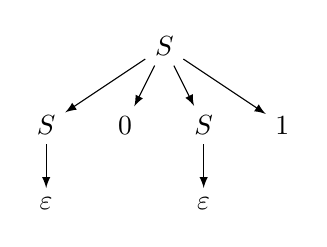
\begin{tikzpicture}
    \node (q_0) at (0,0) {$S$};
    \node (q_1) at (-1.5,-1) {$S$};
    \node (q_2) at (-0.5,-1) {$0$};
    \node (q_3) at (0.5,-1) {$S$};
    \node (q_4) at (1.5,-1) {$1$};
    \node (q_5) at (-1.5,-2) {$\varepsilon$};
    \node (q_6) at (0.5,-2) {$\varepsilon$};
    \draw[->, >=latex] (q_0) -- (q_1);
    \draw[->, >=latex] (q_0) -- (q_2);
    \draw[->, >=latex] (q_0) -- (q_3);
    \draw[->, >=latex] (q_0) -- (q_4);
    \draw[->, >=latex] (q_1) -- (q_5);
    \draw[->, >=latex] (q_3) -- (q_6);
  \end{tikzpicture}
\end{figure}
\end{example}

Le fait suivant est plutôt intuitif. Nous le laissons en exercice pour le
lecteur le plus dubitatif.

\begin{exercise}
  Soit un alphabet $\Sigma$ et une grammaire $G$ sur $\Sigma$. Montrer que
  pour tout $u \in \Sigma^\star$, $u \in \mathcal L_G$ si et seulement s'il
  existe un arbre de dérivation $T$ sur $G$ tel que $\partial T = u$.
\end{exercise}

Supposons qu'on dispose d'un arbre de dérivation $T$ partant d'un non terminal
$S$ et d'un arbre de dérivation $T'$ partant d'un non terminal $A$. Il est alors
possible de \og greffer\fg notre arbre $T'$ à un sommet de $T$ étiqueté par $A$.
On obtient alors un nouveau mot dans notre langage, si $T$ et $T'$ sont des
arbres sur une grammaire du langage (à l'exception près du fait que la racine
de $T'$ peut avoir une étiquette autre que $S$).

Cela nous permet de définir un résultat, analogue à celui du lemme de l'étoile.
Dans le lemme de l'étoile, on a considéré un automate pour dire que celui-ci va
devoir boucler lorsqu'il reconnait un mot suffisamment long. Ici, plutôt que de
considérer les états d'un automate, on considère les symboles utilisés dans
l'arbre de dérivation~: si l'arbre de dérivation est suffisamment haut, alors
il va exister une branche (un chemin de la racine à une feuille) qui va passer
deux fois par le même symbole non terminal, disons $A$. On a alors, pour notre
arbre $T$, un sous-arbre $T'$ dont la racine est $A$ et qui passe par $A$. En
nommant $T''$ le sous-arbre obtenu depuis la deuxième apparition de $A$, on peut
alors greffer $T'$ à $T''$, pour obtenir un nouvel arbre, sur lequel on peut
encore répéter cette opération autant de fois que l'on le souhaite. Au niveau
des mots engendrés par ces itérations d'arbres où $T''$ est remplacé par $T'$,
cela se traduit par le lemme suivant~:

\begin{lemma}[Itération]
  Soit $\Sigma$ un alphabet, $G = (\Gamma,\to,S)$ une grammaire sur $\Sigma$.
  Il existe alors un entier $N$ tel que pour tout $u \in \mathcal L_G$ de
  longueur supérieure à $N$, il existe une décomposition
  \[u = \alpha v \beta w \gamma\]
  telle que
  \[\begin{cases}
  \forall n \in \mathbb N, \alpha v^n \beta w^n \gamma \in \mathcal L_G\\
  |vw| > 0
  \end{cases}\]
\end{lemma}

\begin{proof}
  On sait que $\to$ contient un nombre fini de règles. On définit
  \[d \defeq \max \{|u| \mid (A,u) \in \to\}\]
  et
  \[N \defeq d^{|\Gamma|+2}\]
  D'après les conditions dans la définition d'un arbre de dérivation, on sait
  que pour tout arbre de dérivation sur $G$ et sommet $s$, on a l'inégalité
  \[|d(s)| \leq d\]
  Si un arbre de dérivation $T$ sur $G$ possède une hauteur strictement
  inférieure à $|\Gamma| + 2$, alors (par induction sur la hauteur de l'arbre)
  sa frontière sera de taille strictement inférieure à $d^{|\Gamma| + 2}$, donc
  par contraposition tout arbre de dérivation engendrant un mot $u$ de taille
  supérieure à $N$ doit avoir une hauteur supérieure à $|\Gamma| + 2$. Il existe
  donc une branche $(s_0,\ldots,s_n)$ de longueur supérieure à $|\Gamma| + 2$
  dans cet arbre.

  On utilise maintenant le principe des tiroirs sur la branche
  $(s_0,\ldots,s_{n-1})$ de longueur supérieure à $|\Gamma| + 1$~: il existe
  deux indices $i,j$ tels que $i\neq j$ et $e(s_i) = e(s_j)$. Soient alors les
  arbres $T_0,T_1$ et $T_2$ définis respectivement comme le sous-arbre de $T$
  dont la racine est $s_j$, comme le sous-arbre de $T'$ dont la racine est $e_i$
  et privé de l'arbre $T_0$ et comme $T$ privé de l'arbre $T_0\cup T_1$.

  Soit
  \[A \defeq e(s_i)\]
  On décide de nommer les frontières de nos différents arbres~:
  \[\partial T_0 \defeq \beta \qquad \partial T_1 \defeq vAw \qquad
  \partial T_2 \defeq \alpha A \gamma\]
  Il est dont possible de greffer $T_1$ à $T_2$ un nombre $k$ quelconque de
  fois, puis de greffer $T_0$ à $T_1$, pour obtenir un arbre de dérivation
  valide. On en déduit donc, en prennat la frontière de chacun de ces arbres de
  dérivation itérée~:
  \[\begin{cases}
  \forall n \in \mathbb N, \alpha v^n \beta w^n \gamma \in \mathcal L_G\\
  |vw| > 0
  \end{cases}\]

  On en déduit le résultat souhaité.
\end{proof}

\begin{figure}[ht]
  \centering
  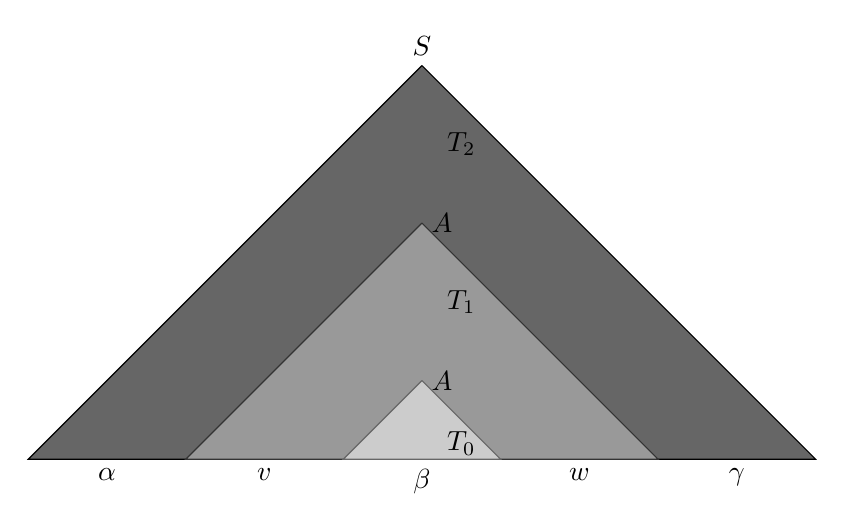
\begin{tikzpicture}
    \node (q0) at (0,0) [above]{$S$};
    \fill[color = black!60] (0,0) -- (-5,-5) -- (5,-5) -- (0,0);
    \draw (0,0) -- (-5,-5) -- (5,-5) -- (0,0);
    \node (q1) at (0.5,-1) {$T_2$};
    \node (q2) at (0,-2) [right]{$A$};
    \fill[color = black!40] (0,-2) -- (-3,-5) -- (3,-5) -- (0,-2);
    \draw[color = black!80] (0,-2) -- (-3,-5) -- (3,-5) -- (0,-2);
    \node (q3) at (0.5,-3) {$T_1$};
    \node (q4) at (0,-4) [right]{$A$};
    \fill[color = black!20] (0,-4) -- (-1,-5) -- (1,-5) -- (0,-4);
    \draw[color = black!60] (0,-4) -- (-1,-5) -- (1,-5) -- (0,-4);
    \node (q5) at (0.5,-4.8) {$T_0$};
    \node (q6) at (-4,-5) [below]{$\alpha$};
    \node (q7) at (-2,-5) [below]{$v$};
    \node (q8) at (0,-5) [below]{$\beta$};
    \node (q9) at (2,-5) [below]{$w$};
    \node (q10) at (4,-5) [below]{$\gamma$};
  \end{tikzpicture}
  \caption{Illustration de la décomposition précédente}
\end{figure}

Un problème se présente cependant, avec les arbres de dérivation. Dans le cas
des dérivations d'un mot, de la forme $S\to^\star u$, on sait qu'il existe en
général de nombreuses dérivations, mais qu'en est-il des arbres de dérivation ?

Une grammaire peut en fait, ou non, posséder un unique arbre de dérivation pour
chaque mot~: c'est ce qu'on appelle une grammaire non ambigüe.

\begin{definition}[Ambigüité]
  Soit $\Sigma$ un alphabet et $G$ une grammaire sur $\Sigma$. On dit que $G$
  est ambigüe lorsqu'il existe deux arbres de dérivation sur $G$ distincts mais
  de même frontière. On dit qu'un langage algébrique $\mathcal L$ est
  inhéremment ambigu s'il n'existe aucune grammaire non ambigüe engendrant
  $\mathcal L$.
\end{definition}

La notion d'ambigüité, ou plutôt de non ambigüité, nous permet de définir une
propriété universelle, analogue au \cref{thm.PU.ind}.

\begin{proposition}[Propriété universelle d'une grammaire non ambigüe]
  Soit $\Sigma$ un alphabet et $G=(\Gamma,\to,S)$ une grammaire non ambigüe sur
  $\Sigma$. Soit un ensemble $X$ et une famille $(f_{A,u})_{(A,u) \in \to}$ de
  fonctions telles que pour tout $(A,u) \in \to$, $f_{A,u} : X^n \to X$ où $n$
  est le nombre de non terminaux appartenant à $u$. Il existe alors une unique
  fonction $f : \mathcal L_G \to X$ telle que pour toute règle
  $A \to u_1A_1\cdots A_nu_{n+1}$ et mots $v_1,\ldots,v_n\in\Sigma^\star$ tels que
  $A_i \to^\star v_i$, on a l'égalité
  \[f(u_1\star v_1\star\cdots\star v_n u_{n+1}) =
  f_{A,u_1A_1\cdots A_nu_{n+1}}(f(v_1),\ldots,f(v_n))\]
\end{proposition}

\begin{proof}
  On raisonne par induction sur la hauteur d'un arbre de dérivation d'un mot
  $u$, en supposant que la racine de l'arbre est un non terminal $A$
  quelconque. Formellement, on prouve qu'il existe une unique fonction dont
  le domaine est l'ensemble des mots s'obtenant par un arbre de dérivation de
  hauteur au plus $n$ depuis un non terminal quelconque~:
  \begin{itemize}
  \item si la dérivation est de la forme $A \to u$ où $u\in\Sigma^\star$, alors
    notre condition est que $f(u) = f_{A,u} \in X$, et cette fonction convient
    bien
  \item supposons qu'un mot $u$ soit obtenu par un arbre de dérivation dont la
    racine est $A$ suivi des sous-arbres $T_1,\ldots,T_k$, où l'on ignore les
    terminaux (on notera $u_1,\ldots,u_{k+1}$ les mots constitués des terminaux
    entre chaque non terminal). On sait alors que $f$ est définie de façon
    unique sur les mots issus de $T_1,\ldots,T_k$ par hypothèse d'induction, et
    alors il existe une unique valeur à $u$ qui est donnée par la condition.
  \end{itemize}

  Ainsi, par induction, tout arbre de dérivation d'un mot est associé à un
  élément de $X$ de sorte de respecter la condition souhaitée, d'où le
  résultat dans le cas des arbres de dérivation dont la racine est $S$.
\end{proof}

\begin{remark}
  En réalité, on aurait pu définir un ensemble $X_A$ pour chaque non terminal
  $A$, ce qui donne une fonction $f$ de codomaine différent pour chaque
  non terminal pris comme symbole de départ.
\end{remark}

Nous profitons de ces définitions pour donner une notion essentielle plus tard~:
le codage de Gödel. Pour cela, on va d'abord introduire le polynôme de Cantor,
qui est une bijection entre $\mathbb N$ et $\mathbb N\times\mathbb N$ très
utilisée en calculabilité.

\begin{definition}[Bijection de Cantor]\label{def.bij.Cantor}
  On appelle bijection de Cantor, ou polynôme de Cantor, la fonction
  \[\begin{array}{ccccc}
  \alpha & : & \mathbb N \times \mathbb N & \longrightarrow & \mathbb N\\
  & & (n,m) & \displaystyle\longmapsto & \left(\sum_{k = 1}^{n+m} k\right)+m
  \end{array}\]
\end{definition}

\begin{exercise}
  Montrer que la bijection de Cantor est effectivement une bijection et
  croissante strictement en chaque coordonnée.
\end{exercise}

L'intérêt de cette fonction est de nous donner un encodage des paires d'entiers
avec les entiers eux-mêmes. On peut en fait généraliser cette idée avec les
$k$-uplets d'entiers, et même les listes d'entiers.

\begin{definition}
  On définit la \ordinalnumeralfeminin{$n$} bijection, $\alpha_n$, par
  récursion sur $n$~:
  \begin{itemize}
  \item la bijection $\alpha_1 : \mathbb N \cong \mathbb N$ est définie par
    l'identité.
  \item si $\alpha_n$ est définie, alors on définit
    \[\begin{array}{ccccc}
    \alpha_{n+1} & : & \mathbb N^{n+1} & \longrightarrow & \mathbb N\\
    & & (p_1,\ldots,p_{n+1}) & \longmapsto &
    \alpha_2(\alpha_n(p_1,\ldots,p_n),p_{n+1})
    \end{array}\]
  \end{itemize}

  On définit aussi la bijection $\alpha_\star : \mathbb N^\star \cong \mathbb N$
  par récursion sur les listes~:
  \begin{itemize}
  \item $\alpha_\star (\varepsilon) = 0$
  \item $\alpha_\star (u\star a) = 1 + \alpha_2(\alpha_\star(u),a)$
  \end{itemize}
\end{definition}

\begin{exercise}
  Montrer que $\alpha_n$ et $\alpha_\star$ sont des bijections croissantes
  strictement en chaque coordonnée.
\end{exercise}

\begin{notation}
  On notera en général $\langle n,m\rangle$ pour $\alpha_n(n,m)$, et de même
  $\langle n_1,\ldots,n_p\rangle$ pour $\alpha_p(n_1,\ldots,n_p)$.
\end{notation}

\begin{definition}[Codage de Gödel d'un langage algébrique]
  Soit $\Sigma$ un alphabet et $G=(\Gamma,\to,V)$ une grammaire non ambigüe sur
  $\Sigma$. Pour chaque $A \in \Gamma$, on numérote les règles $(A,u) \in \to$
  pour les ordonner, on note $e(A,u)$ le numéro de la règle $A,u$. Soit
  $u = u_1A_1\cdots A_nu_{n+1}$ où $u_1,\ldots,u_{n+1}\in\Sigma^\star$, on définit
  \[f_{A,u}(x_1,\ldots,x_n)\defeq \langle e(A,u),x_1,\ldots,x_n\rangle\]
  La fonction obtenue est ce qu'on appelle le codage de Gödel de
  $\mathcal L_G$~:
  \[\ceil{-} : \mathcal L_G \to \mathbb N\]
\end{definition}

\begin{example}
  On fixe une signature du premier ordre $\Delta$ et un ensemble de variables
  du premier ordre $\mathcal X$. On peut définir les formules sur la signature
  $\Delta$ par la grammaire suivante~:
  \begin{align*}
    S &\Coloneq \forall x, S \mid \exists x, S\mid T\\
    T &\Coloneq U \to T \mid U\\
    U &\Coloneq V \lor U \mid V\\
    V &\Coloneq W \land V \mid W\\
    W &\Coloneq \lnot W \mid \top \mid \bot \mid Y = Y \mid
    R^p(Y,\ldots,Y)\mid (S)\\
    Y &\Coloneq x \mid f^p(Y,\ldots,Y)
  \end{align*}
  où $x \in \mathcal X$, $R^p$ décrit l'ensemble des symboles de relation
  d'arité $p$ et $f^p$ les symboles de fonctions d'arité $p$. Les tuples
  $Y,\ldots,Y$ sont des $p$-uplets~: en particulier pour $p = 0$ on a simplement
  $R^0$ (respectivement $f^0$).
  
  On peut vérifier que la grammaire est sans ambigüité. Ainsi, pour une formule
  $\varphi$ donnée, on peut lui associer un entier naturel $\ceil\varphi$, en
  prenant comme numérotation l'ordre dans lequel on a présenté les règles venant
  d'un même non terminal.

  En particulier, lorsque $\Delta$ est la signature de l'arithmétique
  $\mathcal L_{\mathrm{Arith}}$ dont nous avons parlé dans le
  \cref{chp.logpred}, on peut de plus associer à une formule $\varphi$ son
  code de Gödel $\ceil\varphi$, puis le terme dans le langage de l'arithmétique
  $S^{\ceil\varphi}0$. On a ainsi une façon de représenter une formule de
  l'arithmétique à l'intérieur même de l'arithmétique. Nous verrons que ce
  processus est au c\oe ur des théorèmes d'incomplétude de Gödel.
\end{example}

\begin{remark}
  Si l'on parle ici \emphexpr{du} codage de Gödel, c'est en réalité un abus de
  langage. Tout d'abord, ce codage est paramétré par plusieurs choix, dont celui
  de la grammaier et de la numérotation des des règles. De plus, le terme
  \og code de Gödel\fg est informel et recouvre une grande classe de fonctions
  possibles, qui ont pour but d'internaliser les formules de l'arithmétique,
  c'est-à-dire de pouvoir exprimer au sein du langage de l'arithmétique les
  notions liées aux propositions sur l'arithmétique (ce que nous avons présenté
  ici avec le terme $S^{\ceil\varphi}0$). Historiquement, le premier codage de
  Gödel utilisait la décomposition en facteurs premiers, pour encoder un
  tuple $(n_1,\ldots,n_k)$ par l'entier
  $2^{n_1}\times 3^{n_2}\times\cdots \times p_k^{n_k}$ où $(p_n)$ est
  l'énumération canonique des nombres premiers.
\end{remark}

\begin{remark}
  Dans notre description des propositions, nous avons un ensemble infini de
  symboles avec $x \in \mathcal X$. Pour résoudre ça, il suffit de considérer
  $x$ comme un symbole non terminal et la règle
  \[x \Coloneq x_0\mid x_s\;x\]
  décrivant une variable $x_0$ et une fonction injective non surjective
  $x_s : \mathcal X \to \mathcal X$. Ainsi la variable $x_n$ est remplacée par
  la variable $(x_s)^n\;x_0$ et on a alors bien un langage algébrique. Cela
  nous donne d'ailleurs un codage plus explicite des termes (les expressions
  dérivées de $Y$ dans notre grammaire).
\end{remark}

\subsection{Automates à pile}

Dans cette sous-section, l'objectif sera de présenter les automates à pile.
A FAIRE
